\documentclass[a4paper, 11pt]{scrreprt}
\usepackage[utf8]{inputenc}
\usepackage[ngerman]{babel}
\usepackage[T1]{fontenc}
\usepackage{lmodern}
\usepackage{amsmath,amssymb,amstext,amsfonts,mathrsfs, amsthm}
\usepackage{graphicx}
\usepackage{color}

\usepackage{marginnote}

\pagestyle{headings}

\newtheorem{defi}{Definition}[section]
\newtheorem{prop}[defi]{Proposition}
\newtheorem{theorem}[defi]{Theorem}
\newtheorem{coro}[defi]{Corollary}
\newtheorem{lemma}[defi]{Lemma}

\newcommand{\RR}{\mathbb{R}}
\newcommand{\EE}{\mathbb{E}}
\newcommand{\ZZ}{\mathbb{Z}}
\newcommand{\NN}{\mathbb{N}}
\newcommand{\FF}{\mathcal{F}}

\newcommand{\student}[1]{\marginnote{{\normalfont\bf #1}}}

\title{Abschlussarbeit Fallstudien der math. Modellbildung}
\author{Manuela Lambacher, Dominik Otto, Andreas Wiedemann}
\date{\today}

\begin{document}
\parindent 0pt
\maketitle
%\tableofcontents


\chapter{Das Marchenko-Pastur-Gesetz}

\section*{Das Marchenko-Pastur-Gesetz}

Sei \(Y_N\) eine \(N\times M(N)\)-Matrix mit unabhängigen zentrierten Einträgen mit Varianz \(1\),
	\[\sup_{j,k,N} \EE\left[ | Y_N(j,k)|^q\right] = C_q < \infty \qquad \forall q \in \NN\]
und \(M(N) \in \NN\) so, dass
	\[\lim_{N\to\infty} \frac{M(N)}{N} = \alpha \in[1,\infty). \]
Sei weiterhin die Wishart-Matrix gegeben als 
	\[W_N = \frac{1}{N}Y_NY_N^T,\]
und habe die empirische Eigenwertverteilung
	\[L_N = \frac{1}{N} \sum_{j=1}^{N} \delta_{\lambda_j} \]
und das Zustandsdichtemaß \(\overline{L_N} = \EE[L_N]\). Dann gilt die Konvergenz
	\[\overline{L_N} \xrightarrow{\text{w}} f_{\alpha}(x)dx \quad(N\to\infty)\]
im Raum der Wahrscheinlichkeitsmaße auf \(\RR\), wobei
	\[f_{\alpha}(x)=\frac{1}{2\pi x}\sqrt{(x-(1-\sqrt{\alpha})^2_{+}((1+\sqrt{\alpha})^2_{+}} \]

\newpage
\section*{Beweis des Marcenko-Pastur Gesetzes}
Die Konvergenz soll im Folgenden mittels der Momentenmethode gezeigt werden. Als ersten Schritt bringt man \(N^{l+1} \langle \overline{L_N}, x^l \rangle\) in eine Form, die eine weitergehende Untersuchung ermöglicht:
\begin{equation}
\begin{split}
		N^{l+1} &\langle \overline{L_N}, x^l \rangle\ 
		= N^{l+1} \cdot \int x^l \overline{L_N}(dx) 
		= N^{l+1} \cdot \frac{1}{N} \cdot \EE[tr(W^l_N)] 
		= N^l \sum_{j_1,...,j_l = 1}^N \EE\left[\prod_{p = 1}^l W_{j_p,j_{p+1}}\right] \\
		&= N^l \sum_{j_1,...,j_l = 1}^N \EE\left[\prod_{p = 1}^l \frac{1}{N} \sum_{k = 1}^{M(N)} Y_N(j_p,k) \cdot Y_N(j_{p+1},k) \right] \\
		&= \sum_{j_1,...,j_l = 1}^N \EE \left[\left(\sum_{k = 1}^{M(N)} Y_N(j_1,k) \cdot Y_N(j_2,k)\right) \cdot \left(\prod_{p = 2}^l \sum_{k = 1}^{M(N)} Y_N(j_p,k) \cdot Y_N(j_{p+1},k) \right) \right] \\
		&= \sum_{j_1,...,j_l = 1}^N \EE\left[	\prod_{p = 2}^l \sum_{k_1,k_2 = 1}^{M(N)} Y_N(j_1,k_1) \cdot Y_N(j_2,k_1) \cdot Y_N(j_p,k_2) \cdot Y_N(j_{p+1},k_2) \right] \\
		&= (...)~ \text{(es wird analog zum vorherigen Schritt für alle p verfahren)}  \\
		&= \sum_{j_1,...,j_l = 1}^N \sum_{k_1,...,k_l = 1}^{M(N)} \EE[Y_N(j_1,k_1) Y_N(j_2,k_1) Y_N(j_2,k_2) Y_N(j_3,k_2) ... Y_N(j_l,k_l) Y_N(j_1,k_l)]\\
 &= \sum_{s_1,s_2 = 1}^l \sum_{\substack{J:v(J)=s_1\\ K:v(K)=s_2 }} \EE[Y_N(J,K)]
\end{split}
\end{equation}
wobei 
\begin{align*}
	&J=(j_1,j_2,j_2,...,j_l,j_l,j_1), K=(k_1,k_1,...,k_l,k_l),\\
	&v: \NN^{2l}\to \NN,\ v(X) := \text{Anzahl der verschiedenen Indizes in X}
\end{align*}
\\
Die einzelnen Summanden können also als Eulergraphen auf \(s_1+s_2 \)verschiedenen Knoten und \(2l\) Kanten zwischen der Menge der k-Knoten und der j-Knoten für alle Paare $ (j_i, k_i), (j_{i+1},k_i) $ interpretiert werden.\\
Setze \(s = s_1+s_2\), dann ergeben sich folgende drei Fälle:
\begin{itemize}
	\item \(s < l+ 1\)\\
		\begin{equation}
			\begin{split}
			\EE[Y_N(J,k)] &\leq \prod_{n=1}^l \left(\sup_{j,k,N}\EE\left[|Y_N(j,k)|^l\right]\right)^{\frac 1 l} \\
			& = \prod_{n=1}^l C_l^{\frac 1 l} = C_l
			\end{split}
			\end{equation}
	Außerdem gilt: 
		\begin{align}
			\#\{J: v(J)=s_1\} &\leq \begin{pmatrix} N \\ s_1 \end{pmatrix} s_1^l \leq N^{s_1}s_1^l \\
			\#\{K: v(K)=s_2\} &\leq \begin{pmatrix} M(N) \\ s_2 \end{pmatrix} s_2^l \leq M(N)^{s_2}s_2^l
		\end{align}
	Somit ergibt sich aus \((1.2) - (1.4)\): 
	\begin{equation}
		\frac {1}{N^{l+1}} \sum_{\substack{J:v(J)=s_1\\ K:v(K)=s_2 }} \EE[Y_N(J,K)] < C_l (l+1)^l \frac{N^{s_1} M(N)^{s_2}}{N^{l+1}} \xrightarrow{N\to\infty} 0
	\end{equation}
		
	\item \(s> l+1\) \\
		Nach Lemma aus der Vorlesung existiert in diesem Fall eine einfache, echte Kante. Da die Matrixeinträge unabhängig sind, kann der Erwartungswert für diesen Matrixeintrag ausgeklammert werden. Alle Einträge sind jedoch zentriert, und damit folgt direkt \(\EE[Y_N(J,K)]=0\).
	\item \(s=l+1\)\\
		Die verbliebenen Graphen auf \(l+1\) verschiedenen Knoten haben die Struktur von Doppelbäumen und sollen im Weiteren genauer untersucht werden.\\
\end{itemize}		
Zusammenfassung: Zu \(\lim_{N\to\infty} \langle \overline{L_N}, x^l \rangle \) tragen nur die Graphen auf $ l+1 $ verschiedenen Knoten bei:

\begin{equation}
\begin{split}
\beta_l:= \lim_{N\to\infty} \langle \overline{L_N}, x^l \rangle &= \lim_{N\to\infty} \dfrac{1}{N^{l+1}} \sum_{s_1,s_2 = 1}^l \sum_{\substack{J:v(J)=s_1\\ K:v(K)=s_2 }} \EE[Y_N(J,K)]\\ &= \lim_{N\to\infty} \dfrac{1}{N^{l+1}}\sum_{J,K: v(J)+v(K) = l+1} \EE[Y_N(J,K)]  
\end{split}
\end{equation}\\

\subsection*{Berechnung der $ \beta_l $ mittels Catalanpfade}
Die Doppelbaumstruktur dieser Graphen lässt sich wie folgt nutzen:\\
Wähle für einen Doppelbaum \(r\) Knoten aus den \(k\)-Knoten und \(l+1-r\) Knoten aus den \(j\)-Knoten. Dann gilt:
\begin{equation}
	\begin{split}
	\sum_{J,K: v(J)+v(K) = l+1} \EE[Y_N(J,K)] = &\sum_{r=1}^{l}\begin{pmatrix} N\\ l+1-r\end{pmatrix} (l+1-r)! \begin{pmatrix} M(N)\\r\end{pmatrix} r! \\
	&\cdot \#\{\text{Doppelbäume mit }l+1-r\ j\text{-Knoten und } r\ k\text{-Knoten}\} \\
	\end{split}
\end{equation}

Ein Doppelbaum mit \(r\  k\)-Knoten und \((l+1-r)\ j\)-Knoten kann nun in folgender Weise als Catalan-Pfad der Länge \(l\) interpretiert werden:\\\\
Wähle als Wurzel des Baumes einen \(j\)-Knoten und gliedere den Baum in Ebenen, wobei die Wurzel in der 0.Ebene liegt. Die \(k\)-Knoten liegen also in ungeraden Ebenen, die \(j\)-Knoten in geradenen Ebenen. Verweise jede Kante mit einer Richtung, sodass bei jeder Doppelkante eine Kante von dem Knoten wegführt und eine zu ihm hinführt. Durchlaufe den Baum mit Hilfe der Tiefensuche und nummeriere die Kanten in der Reihenfolge, wie sie hierbei durchlaufen werden. Konstruiere den Catalan-Pfad wie folgt:
\begin{itemize}
	\item Wird ein Knoten zum ersten Mal erreicht: \((+1)\)
	\item Kehrt man zu einem bereits besuchten Knoten zurück :\((-1)\)
	
\end{itemize}
Da der Baum durch Tiefensuche durchlaufen wird, gibt die Entfernung eines Knotens zur Wurzel die Anzahl der nötigen Schritte wieder, die benötigt werden, um ihn zum ersten Mal zu erreichen. Da die \(j\)-Knoten in den geraden Ebenen und die \(k\)-Knoten in den ungeraden Ebenen liegen, ergibt sich, dass sich die \(j\)-Knoten stets auf den geraden Niveaus und die \(k\)-Knoten stets auf den ungeraden Niveaus des Catalan-Pfades befinden. 

\begin{figure}[htpb]
	\centering
	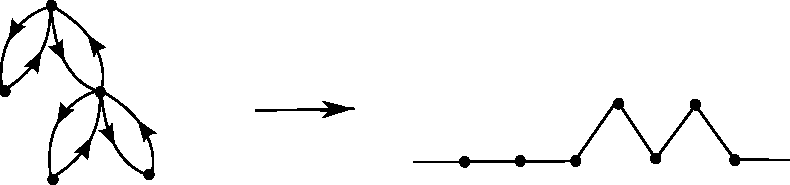
\includegraphics[width=1.00\textwidth]{Catalan-Pfad.pdf}
	\caption{Doppelbaum auf 5 Knoten und dem zugehörigen Catalan-Pfad} 
\end{figure}

Die Abbildung von den Doppelbäumen auf die Catalanpfade ist eine Bijektion:
\begin{itemize}
 \item[•]Wohldefiniertheit: Da der Graph eulersch ist, ist $ \sum_{i=1}^{2l} $ =0; Der Graph ist immer auf oder überhalb des 0.Niveaus, ansonsten würde es ein m geben, sodass $ \sum_{i=1}^{2m-1}s^{i}=-1, ~\sum_{i=1}^{2m}s^{i}=0, ~ s_{2m-1}=-1  $. Also könnte ein Doppelbaum mit Knoten {1,2,...2m} konstruiert werden, und da $ s_{2m-1}=-1  $ gilt, würde eine Kante von diesem Knoten zurück zu einem der ersten 2m Knoten gehen, was dem Aufbau eines Doppelbaums widersprechen würde. Insgesamt wurde also tatsächlich ein Catalanpfad konstruiert. 
 \item[•] Surjektivität: Starte bei der Wurzel. Füge für jede Aufstiegskante einen Knoten in die nächst höhere Ebene und eine Kante als Verbindung hinzu. Füge für jede Abstiegskante eine Kante in die nächst niedrigere Ebene hinzu, bis die Doppelbaumstruktur vollständig ist. Damit ist jeder Catalanpfad Urbild eines Doppelbaums. 
\item[•] Injektivität: kann analog zur Übung durch rekursives Entfernen von identischen Kanten gezeigt werden.\\
\end{itemize}
Damit ist die Anzahl der Doppelbäume in (1.7) gleich der Anzahl der dazugehörigen Catalanpfade.\\
Die betrachteten Doppelbäume haben nach (1.7) ein kombinatorisches Gewicht von 
	\begin{equation}
		\begin{pmatrix} N\\ l+1-r\end{pmatrix} (l+1-r)! \begin{pmatrix} M(N)\\r\end{pmatrix} r!
	\end{equation}
Für N hinreichend groß ist dies genähert \(N^{l+1-r}M(N)^r\). Damit gilt:
	\begin{equation}
		\frac {1}{N^{l+1}} N^{l+1-r}M(N)^r =~ \left( \dfrac{M(N)}{N}\right)^{r}\to \alpha^r
	\end{equation}
und schließlich folgt mit (1.6):
	\begin{align*}
		\beta_l &:= \lim_{N\to\infty} \langle \overline{L_N}, x^l \rangle\\
		&= \lim_{N \to \infty} \sum_{J,K: v(J)+v(K) = l+1} \dfrac{1}{N^{l+1}}\EE[Y_N(J,K)]\\
		&= \lim_{N \to \infty} \sum_{r=1}^{l} \dfrac{1}{N^{l+1}} \begin{pmatrix} N\\ l+1-r\end{pmatrix} (l+1-r)! \begin{pmatrix} M(N)\\r\end{pmatrix} r!	\cdot \#\{p_r \}\\
		&= \sum_{r=1}^{l} \sum_{p_{r} \in C_{l}} \alpha^{r} = \sum_{p\in C_l} \alpha^r
	\end{align*}
wobei \(r=\#\{\text{Abstiege von ungeraden auf gerade Niveaus in } C_l\}\), und \(p_r\) Catalan-Pfad mit \(r\) entsprechenden Abstiegen.\\

%!!! Explizite Formel für die Anzahl der $ p_r $ gefunden: \[ \binom{l-1}{r} \binom{l}{r} \frac{1}{r+1} \]
%Wer Spaß dran hat, kann sie beweisen. Ansonsten lassen wir sie raus, wir brauchen sie ja nicht.\\

\subsection*{Relation für $ \beta_l $}
Zu zeigen ist: Mit \(\beta_0 :=1, \gamma_0:=1 \) und
\begin{equation*}
		\gamma_l:=\sum_{p\in C_l} \alpha^{l-r} \qquad (l\geq 1)
\end{equation*}
gelten die Relationen
\begin{equation}
	\label{eq:beta_l}
	\beta_l = \alpha\gamma_l=\alpha\sum_{r=0}^{l-1}\beta_r \gamma_{l-1-r} ~~\forall l \geq 1
\end{equation}
(\(l-r\) ist dabei die Anzahl der Abstiegskanten von geraden auf ungerade Niveaus im Catalan-Pfad.)
\begin{itemize}

\item
Betrachte die Position im Pfad, an der zum ersten Mal die \(0\) erreicht wird. Diese ist immer gerade, da die \(0\) genau dann erreicht wird, wenn man im zugehörigen Doppelbaum zur Wurzel zurückkehrt. Sei also \(2j\), \(j\in\{1,...,l\}\), diese Position. \\
Teile nun den Pfad in einen vorderen Teil \(P_1\) der Länge \(2j\) und einen hinteren Teil \(P_2\) der Länge \(2l-2j\). In dem erzeugenden Baum entspricht \(P_1\) dem äußersten Teilbaum, \(P_2\) dem restlichen Baum. \(P_2\) ist also ein beliebeiger Catalan-Pfad. \(P_1\) hat die besondere Struktur, dass die \(0\) erst an letzter Position erreicht wird, die erste und letzte Kante sind somit als Auftsiegs- bzw. Abstiegskante festgelegt und können für die kombinatorische Analyse vernächlässigt werden. Löscht man diese beiden Kanten und subtrahiert \(1\) von allen Elementen von \(P_1\), erhält man einen neuen Pfad \(\tilde{P}_1\), der ein beliebiger Catalan-Pfad der Länge \(2j-2\) ist. Dies folgt direkt aus der Struktur des Doppelbaumes: \(\tilde{P}_1\) entspricht dem äußersten Teilbaum ohne die ursprüngliche Wurzel, wodurch man einen neuen, beliebigen Doppelbaum erhält. \\
Die geraden/ungeraden Niveaus im ursprünglichen Pfad sind in \(\tilde{P}_1\) ungerade/gerade (Durch die Verschiebung um \(1\) nach unten). \(r\) und \(l-r\) haben sich also genau vertauscht.
\begin{figure}[htpb]
	\centering
	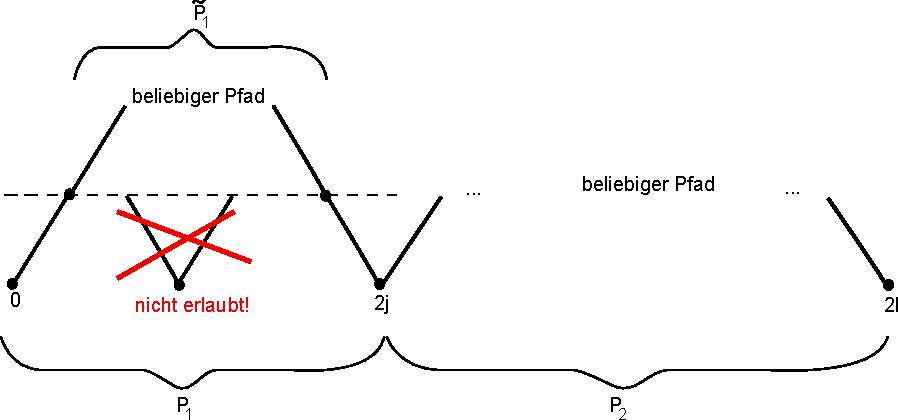
\includegraphics[width=1.00\textwidth]{Rekursion-Visualisierung.pdf}
	\caption{Schematische Darstellung der Rekursion}
\end{figure}
Damit ergibt sich aus den Definition für \(\beta_l\) und \(\gamma_l\) die Formel:
\begin{equation}
	\begin{split}
		\beta_l &= \alpha\sum_{j=1}^{l-1}\gamma_{j-1}\beta_{l-j} = \alpha\sum_{j=0}^l \gamma_j\beta_{l-j-1}\\
		&=\alpha\sum_{k=0}^l \beta_k\gamma_{l-1-k}
	\end{split}
\end{equation}
Das zusätzliche \(\alpha\) wird in der Formel durch das Löschen der gewichteten Abwärtskante in \(P_1\) hervorgerufen.\\


\item $ \gamma $ wird analog dargestellt: Im Gegensatz zu vorher tragen nun die Abwärtskanten von gerade zu ungerade zum Gewicht von $ \alpha $ bei. Sei \(2j\), \(j\in\{1,...,l\}\), die Position, an der zum ersten Mal die \(0\) erreicht wird. \\
Teile wiederum den Pfad in einen vorderen Teil \(P_1\) der Länge \(2j\) und einen hinteren beliebigen Catalanpfad \(P_2\) der Länge \(2l-2j\). In \(P_1\) sind wieder die erste und letzte Kante festgelegt. Beim Löschen dieser Kante werden die Ebenen vertauscht. \\
Anders als bei den $ \beta_l $ wurde durch das Löschen der Abwärtskante allerdings kein $ \alpha $ verloren, da nun lediglich die Abwärtskanten von gerade zu ungerade das Gewicht $ \alpha $ haben.\\ 
Damit gilt: 
\begin{equation}
	\begin{split}
		\gamma_l &=\sum_{k=0}^l \beta_k\gamma_{l-1-k} \\
		&= \dfrac{\beta_l}{\alpha}
	\end{split}
\end{equation}\\

\end{itemize}

\subsection*{Verallgemeinerten Momente von $ f_\alpha $}
Man betrachtet \[xf_{\alpha}(x)=\frac{1}{2\pi}\sqrt{(x-(1-\sqrt{\alpha})^2_{+}((1+\sqrt{\alpha})^2_{+}} \] und vergleicht es mit dem aus der Vorlesung bekanntem Halbkreisgesetz \[ \sigma(x)= \frac{1}{2 \pi} \sqrt{(4-x^2)_+}\]
Dabei wird ersichtlich, dass $ xf_\alpha $ als ein modifizierter Halbkreis beschrieben werden kann: Es ist null außerhalb seiner Schnittpunkte mit der x-Achse, $ xf_\alpha(1+\alpha +x)=xf_\alpha (1+\alpha -x) $, d.h. symmetrisch um seinen "'Mittelpunkt"' $ 1+\alpha $. Man kann den Graph der Funktion somit als einen um $ \alpha +1 $ verschobenen und um einen konstanten Faktor nach oben verzerrten Halbkreis beschreiben. Auch in der nun folgenden Rechnung wird durch Substitution wieder das Halbkreisgesetz erreicht. \\
Anmerkung: Berechnung liefert $ \int_{\RR} f_\alpha(x)dx=1 $, $ f_\alpha $ ist ein Wahrscheinlichkeitsmaß.\\\\

\textbf{Beweis der Formel für $ Q_n$}
\begin{align*}
	Q_n :=& \alpha^{-1-n/2}\int_{\RR} f_{\alpha}(x)x(x-\alpha -1)^n\,\mathrm{d}x \\
	 =& \frac{1}{2\pi}\alpha^{-1-n/2} \int_{(1-\sqrt{\alpha})^2}^{(1+\sqrt{\alpha})^2} \sqrt{(x-(1-\sqrt{\alpha})^2)((1+\sqrt{\alpha})^2-x)} (x-\alpha -1)^n \,\mathrm{d}x\\
	=& \frac{1}{2\pi}\alpha^{-1-n/2} \int_{(1-\sqrt{\alpha})^2}^{(1+\sqrt{\alpha})^2} \sqrt{-\alpha^2+2\alpha x+2\alpha -x^2+2x-1}(x-\alpha-1)^n \,\mathrm{d}x\\
	\displaybreak
	\overset{x=y+\alpha+1}{=}& \frac{1}{2\pi}\alpha^{-1-n/2} \int_{-2\sqrt{\alpha}}^{2\sqrt{\alpha}} \sqrt{4\alpha -y^2} y^n \,\mathrm{d}y\\
	\overset{y=2\sqrt{\alpha}z}{=}& \frac{1}{2\pi}\alpha^{-1-n/2} \cdot 2^n \alpha^{n/2}\cdot4\sqrt{\alpha}\int_{-1}^{1} \sqrt{1-z^2}z^n \,\mathrm{d}z = \frac{2}{\pi} \cdot 2^n\int_{-1}^{1} \sqrt{1-z^2}z^n\,\mathrm{d}z \\
	\overset{\text{Übung 1}}{=}& \sigma(z^n) = \begin{cases} 0, &n\text{ ungerade}\\
	C_{\frac n 2}, &n\text{ gerade} \end{cases}
\end{align*}

Also \begin{equation}
Q_n=\begin{cases} 0, &n\text{ ungerade}\\
	C_{\frac n 2}, &n\text{ gerade} \end{cases}
\end{equation}\\

Nachdem $\lbrace \alpha^{-1-n/2} x(x-\alpha -1)^n \vert n \in \NN_{0}\rbrace \cup \lbrace 1 \rbrace$ ebenso eine Basis aller Polynome darstellt wie $ \lbrace x^l \vert l \in \NN_{0} \rbrace $, ist $ f_{\alpha} $ durch die $ Q_n $ und $ \int_{\RR} f_{\alpha}(x)dx $ genauso bestimmt wie durch die normalen Momente. 

\begin{theorem}
Sei $ \mu \in \mathcal{M}(\RR) $ mit $ m_l (\mu)=\int x^l \mu(dx) < \infty~ \forall l \in \NN_{0} $\\
Dann ist $ \mu $ das einzige Wahrscheinlichkeitsmaß mit diesen Momenten, wenn die Potenzreihe 
\[\sum_{l=0}^\infty m_l(f_\alpha) \frac{z^l}{l!}\]
einen positiven Konvergenzradius besitzt.
\end{theorem}

Da die Momente $ m_l $ endliche Linearkombinationen der verallgemeinerten Momente sind, wird das Theorem jetzt auf die $ Q_n $ angewandt.\\
Also ist zu zeigen: $ Q_n< \infty $ (folgt direkt aus (1.13)) und $ \sum_{n=0}^{\infty} Q_n \dfrac{z^n}{n!}$ besitzt positiven Konvergenzradius.\\
\[ \sum_{n=0}^{\infty} Q_n \dfrac{z^n}{n!}= \sum_{n=0}^{\infty} a_n z^n\]\\
wobei \[ a_n=\begin{cases} 0, &n\text{ ungerade}\\
	\dfrac{C_{\frac n 2}}{n!}=((\frac{n}{2}+1)!\frac{n}{2}!)^{-1}, &n\text{ gerade} \end{cases} \]
	nach der Definition der Catalanzahlen.
	Wurzelkriterium für Konvergenzradius ergibt: 
	\[(\frac{n}{2}+1)!\frac{n}{2}! \geq 1 \Rightarrow \vert a_n \vert \leq 1 \Rightarrow \]
	\[ r=(\limsup_{n \to \infty} \sqrt[n]{\vert a_n} \vert )^{-1} >1 \]

Damit ist das Wahrscheinlichkeitsmaß $f_\alpha  $ eindeutig durch seine verallgemeinerten Momente bestimmt.

\subsection*{Verallgemeinerte Momente von $ \overline{L_N} $ für $ N \to \infty $}
Nachdem bereits $ f_\alpha $ durch seine Momente bestimmt wurde, wird im folgenden Abschnitt der Grenzwert der verallgemeinerten Momente von $ \overline{L_N} $ untersucht. Hierfür werden die Ergebnisse für $ \beta_l $ benötigt.\\
\begin{equation}
R_n:=\lim_{N \to \infty} \alpha^{-1-n/2} \int_{\RR}\overline{L_{N}}(dx)x(x-\alpha-1)^{n} 
\end{equation}
Anwendung des binomischen Lehrsatzes ergibt:
\begin{equation}
 \begin{split}
 R_n =& \alpha^{-1-n/2} \lim_{N \to \infty} \int_{\RR}\overline{L_{N}}(dx)x \sum_{k=0}^n \begin{pmatrix} n\\k\end{pmatrix} x^{n-k}(-\alpha -1)^k \\
 =& \alpha^{-1-n/2} \lim_{N \to \infty} \langle \overline{L_{N}}, \sum_{k=0}^n \begin{pmatrix} n\\k\end{pmatrix} x^{n+1-k}(-\alpha -1)^k \rangle \\
 =& \alpha^{-1-n/2}\sum_{k=0}^n \begin{pmatrix} n\\k\end{pmatrix} (-\alpha -1)^k \beta_{n+1-k}
 \end{split}
\end{equation}

wegen $\beta_l = \lim_{N\to\infty} \langle \overline{L_N}, x^l \rangle$ und der Linearität des Integrals.\\

Um die Rekursionsformel zu zeigen benötigt man folgende Formel:
\begin{equation}
\label{eq:binom}
	\sum_{n= t}^{t+u} \binom{m-n}{m-u-t} \binom{n}{t} = \binom{m+1}{u}~~\forall\ t: \ 0\leq t \leq m-u
\end{equation}
\textbf{Beweis von (1.16)}  
Man führt den Beweis anschaulich anhand des Pascalschen Dreiecks durch. Jeder Binomialkoeffizient wird mit einem Knoten im Dreieck identifiziert, sein Wert ist gleich der Anzahl der Pfade, die zu ihm führen. \\
Betrachte den Punkt $ \binom{m+1}{m+1-u} $. Für ein festes $t+1$ sodass $~m-u+1\geq t+1 \geq 1$ definiert man  eine Diagonale \[T=\left\lbrace  \binom{n+1}{t+1}~\vert n+1 \geq t+1 \right\rbrace  \] Jeder Pfad von $ \binom{0}{0} $ zu $ \binom{m+1}{m+1-u} $ muss diese Diagonale überqueren. \\Sei $ \binom{n+1}{t+1} $ der Punkt, an dem der Pfad $ T $ zum ersten Mal berührt. Der vorhergehende Schritt ist damit eindeutig festgelegt, er muss von $ \binom{n}{t} $ gekommen sein, sonst wäre er bereits auf $ T $ gewesen.\\ 
Man summiert nun über alle möglichen ersten Punkte auf $ T $. Die dazugehörigen Pfade im Pascalschen Dreieck werden in zwei Teilpfade unterteilt. Der erste, um $ \binom{n+1}{t+1} $ zu erreichen, wobei der letzte Schritt vorgegeben ist. Es bleiben $ \binom{n}{t} $ Möglichkeiten für diesen Abschnitt.\\
Der zweite Teilpfad zwischen dem Punkt auf $ T $ und dem Ziel hat das kombinatorische Gewicht von $\binom{m-n}{m-u-t}$\\
Nun muss man noch betrachten, welches das größtmögliche n+1 ist, das noch einen Beitrag zu der Summe liefert. Dies ist der Fall, wenn \[ \binom{m+1-n-1}{m+1-u-t-1}=1,  \] d.h. es gibt nur noch eine Möglichkeit für den zweiten Teilpfad. Dies ist gleichbedeutend mit $ m-n=m-u-t $.\\Insgesamt wurde gezeigt:
\[ \sum_{n=t}^{t+u}\binom{m-n}{m-u-t} \binom{n}{t}= \binom{m+1}{m+1-u}=\binom{m+1}{u} \]

\begin{figure}[htpb]
	\centering
	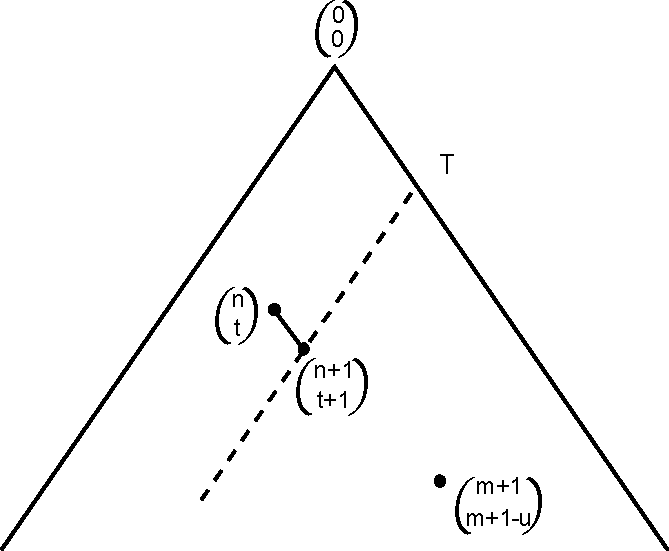
\includegraphics[width=0.45\textwidth]{Parsevalsches-Dreieck.pdf}
	\caption{Darstellung von \ref{eq:binom}}
\end{figure}


\textbf{Beweis der Rekursionsformel}\\\\
Nun betrachtet man:
\begin{align*}
\sum_{n=0}^m R_{m-n} R_n 
&= \sum_{n=0}^m \sum_{k=0}^{m-n} \binom{m-n}{k} (-\alpha -1)^k \beta_{m-n+1-k} \alpha^{-1-\frac{m-n}{2}} \sum_{l=0}^n \binom{n}{l} (-\alpha -1)^l \beta_{n+1-l} \alpha^{-1-\frac{n}{2}} \\
&= \alpha^{-1-\frac{m}{2}} \sum_{n=0}^m \sum_{l=0}^n \sum_{k=0}^{m-n} \binom{m-n}{k}  \binom{n}{l} (-\alpha -1)^{k+l} \beta_{m-n+1-k} \gamma_{n+1-l}	
\end{align*}

Der Index $k$ wird anschließend durch $u:=k+l$ ersetzt.

\[\sum_{n=0}^m R_{m-n} R_n = \alpha^{-1-\frac{m}{2}} \sum_{n=0}^m \sum_{l=0}^n \sum_{u=l}^{m+l-n} \binom{m-n}{u-l}  \binom{n}{l} (-\alpha -1)^u \beta_{m-n+1+l-u} \gamma_{n+1-l}\]

Mit $t:=n-l$ kann $l$ umgeschrieben werden. Die weiteren Umformungen gelten aufgrund der Eigenschaften des Binomialkoeffizienten und $ \gamma_i=\alpha^{-1} \beta_i ~\forall i\geq1$.

\begin{align*}
\sum_{n=0}^m R_{m-n} R_n 
&= \alpha^{-1-\frac{m}{2}} \sum_{n=0}^m \sum_{t=0}^n \sum_{u=n-t}^{m-t} \binom{m-n}{u-n+t}  \binom{n}{t} (-\alpha -1)^u \beta_{m+1-u-t} \gamma_{1+t} \\
&= \alpha^{-1-\frac{m}{2}} \sum_{t=0}^m \sum_{u=0}^{m-t} \sum_{n=t}^{u+t} \binom{m-n}{u-n+t}  \binom{n}{t} (-\alpha -1)^u \beta_{m+1-u-t} \gamma_{1+t} \\
&= \alpha^{-1-\frac{m}{2}} \sum_{u=0}^{m+1} \sum_{t=0}^{m-u} (-\alpha -1)^u \beta_{m+1-u-t} \gamma_{1+t} \sum_{n=t}^{u+t} \binom{m-n}{m-u-t}  \binom{n}{t}
\end{align*}

Mit Formel (1.16) gilt schließlich:

\begin{align*}
\sum_{n=0}^m R_{m-n} R_n 
&= \alpha^{-1-\frac{m}{2}} \sum_{u=0}^{m+1} \sum_{t=0}^{m-u} (-\alpha -1)^u \beta_{m+1-u-t} \gamma_{1+t} \binom{m+1}{u} \\
&= \alpha^{-1-\frac{m}{2}} \sum_{u=0}^{m+1} \binom{m+1}{u} (-\alpha -1)^u \sum_{t=0}^{m-u} \beta_{m+1-u-t} \gamma_{1+t}
\end{align*}

Durch die Substitution $r := m+1-u-t$ und die Anwendung von Formel (\ref{eq:beta_l}) und (1.15) ergibt sich Folgendes:

\begin{align*}
\sum_{n=0}^m R_{m-n} R_n
=& \alpha^{-1-\frac{m}{2}} \sum_{u=0}^{m+1} \binom{m+1}{u} (-\alpha -1)^u \left( \sum_{r=0}^{m+1-u} \beta_r \gamma_{m+2-u-r} - \beta_0 \gamma_{m+2-u} \right) \\
=& \alpha^{-1-\frac{m}{2}} \sum_{u=0}^{m+1} \binom{m+1}{u} (-\alpha -1)^u \left( - \beta_{m+2-u} + \sum_{r=0}^{m+2-u} \beta_r \gamma_{m+2-u-r} - \alpha^{-1} \beta_{m+2-u}\right) \\
=& \alpha^{-1-\frac{m}{2}} \sum_{u=0}^{m+1} \binom{m+1}{u} (-\alpha -1)^u \left(\frac{1}{\alpha} \beta_{m+3-u} - \dfrac{\alpha +1}{\alpha}\beta_{m+2-u} \right) \\
=& \alpha^{-1-\frac{m}{2}} \sum_{u=0}^{m+2} \binom{m+1}{u} (-\alpha -1)^u \frac{1}{\alpha} \beta_{m+3-u} \\
&- \alpha^{-1-\frac{m}{2}} \sum_{u=0}^{m+1} \binom{m+1}{u} (-\alpha -1)^u \dfrac{\alpha +1}{\alpha}\beta_{m+2-u} \\
=& \alpha^{-1-\frac{m}{2}} \sum_{u=0}^{m+2} \left( \binom{m+2}{u} -\binom{m+1}{u-1} \right) (-\alpha -1)^u \frac{1}{\alpha} \beta_{m+3-u} \\
&- \alpha^{-1-\frac{m}{2}} \sum_{u=0}^{m+1} \binom{m+1}{u} (-\alpha -1)^u \dfrac{\alpha +1}{\alpha}\beta_{m+2-u} \\
=& R_{m+2} - \alpha^{-2-m/2}\sum_{u=0}^{m+2} \binom{m+1}{u-1}(-\alpha-1)^u\beta_{m+3-u} \\
\displaybreak
&- \alpha^{-2-m/2}(1+\alpha)\sum_{u=0}^{m+1}\binom{m+1}{u}(-\alpha-1)^u\beta_{m+2-u} \\
=& R_{m+2} + \alpha^{-2-m/2}(1+\alpha)\sum_{i=0}^{m+1} \binom{m+1}{i}(-\alpha-1)^i\beta_{m+2-i} \\
&- \alpha^{-2-m/2}(1+\alpha)\sum_{u=0}^{m+1}\binom{m+1}{u}(-\alpha-1)^u\beta_{m+2-u}
\end{align*}
 Also gilt: 
\begin{equation}
\sum_{n=0}^m R_{m-n} R_n= R_{m+2}
\end{equation}\\



\subsection*{Beweis der schwachen Konvergenz}


Nun soll gezeigt werden, dass $ R_m=Q_m $:\\
Es wird überprüft, dass $ R_0=Q_0 $ und $ R_1=Q_1 $, sowie dass die weiteren Folgenglieder von $ Q_m $ durch die gleiche Rekursionsformel (1.17) gebildet werden können. Daraus folgt unmittelbar $ R_m=Q_m ~ \forall m \in \NN_0$ \\

\begin{itemize}
\item $ R_0=Q_0 $, $ R_1=Q_1 $: 
\begin{align*}
\beta_1=& \alpha \beta_0 \gamma_0 = \alpha \\
\beta_2=& \alpha \beta_0 \gamma_1 + \alpha \beta_1 \gamma_0 = \alpha \gamma_1 + \alpha \beta_1 = \beta_1 + \alpha \beta_1  \\
R_0 =& \lim_{N \to \infty} \alpha^{-1} \int_{\RR}\overline{L_{N}}(dx)x = \dfrac{\beta_1}{\alpha}=1 \\
R_1 =& \alpha^{\frac{3}{2}} \lim_{N \to \infty}\int_{\RR}\overline{L_{N}}(dx)(x^2 - (\alpha +1)x)= \alpha^{\frac{3}{2}} (\beta_2 - (\alpha+1)\beta_1)=0 \\
Q_0=& C_0 =1, ~~Q_1=0
\end{align*}

\item Rekursion für $ Q_m: $
\begin{align*}
\text{m ungerade:}& \sum_{n=0}^m Q_{m-n}Q_n= Q_0 \underbrace{Q_m}_{\substack{=0}} + \underbrace{Q_1}_{\substack{=0}}Q_{n-1}+....= 0=Q_{m+2}\\
\text {m gerade:}&~ Q_{m+2}= C_{\frac{m}{2}+1}= \sum_{k=0}^{\frac{m}{2}} C_k C_{\frac{m}{2}-k}=\sum_{k=0}^{\frac{m}{2}} Q_{2k}Q_{m-2k}=\sum_{n=0}^{m}Q_n Q_{m-n}
\end{align*}
wobei der letzte Schritt aus $ Q_n Q_{m-n}=0 $ für $ n=2k+1 $ folgt.\\
\end{itemize}
Mit folgendem Theorem aus der Vorlesung kann das Marchenko-Pastur-Gesetz nun bewiesen werden.

\begin{theorem}
Sei \((\mu_n)_{n \in \NN}\) eine Folge in $\mathcal{M}(\RR)$ mit endlichen Momenten und $\mu \in \mathcal{M}(\RR)$ eindeutig durch seine Momente bestimmt. Dann gilt:
\[\forall l \in \NN_0: m_l(\mu_n) \rightarrow m_l(\mu) \Rightarrow \mu_n \overset{W}{\rightarrow} \mu\]
\end{theorem}

Die Voraussetzungen dieses Theorems werden nun überprüft.
\begin{itemize}
\item $ \forall l \in \NN_0: m_l(\mu_n) \to m_l(\mu) $\\
Für $l \geq 1$ existieren $\lambda_0,...,\lambda_{l-1} \in \RR$, sodass $x^l = \sum_{n=0}^{l-1} \lambda_n x (x-\alpha-1)^n$. Daraus folgt:
\begin{align*}
\forall l \in \NN: \lim_{N \to \infty} m_l(\overline{L_{N}}) 
&= \lim_{N \to \infty} \int_\RR x^l \overline{L_{N}}(dx)
= \lim_{N \to \infty} \int_\RR \sum_{n=0}^{l-1} \lambda_n x (x-\alpha-1)^n \overline{L_{N}}(dx) \\
&= \sum_{n=0}^{l-1} \lambda_n \lim_{N \to \infty} \int_\RR x (x-\alpha-1)^n \overline{L_{N}}(dx) \\
&= \sum_{n=0}^{l-1} \tilde{\lambda_n} R_n
= \sum_{n=0}^{l-1} \tilde{\lambda_n} Q_n = m_l(f_\alpha)
\end{align*}
Wobei $ \tilde{\lambda_n}= \lambda \alpha ^{1+n/2}$\\

Für den Fall l = 0 erhält man:
\[\lim_{N \to \infty} m_0(\overline{L_{N}}) 
= \lim_{N \to \infty} \int_\RR \overline{L_{N}}(dx) = 1 
= \int_\RR f_\alpha(x)dx\]
da $ \overline{L_N} $ nach Vorlesung ebenfalls ein Wahrscheinlichkeitsmaß ist.

\item Es wurde bereits gezeigt, dass $ f_\alpha $ eindeutig bestimmt ist. 
\item Es bleibt zu zeigen, dass $ R_n $ endlich ist $ \forall n \in \NN_0 $. Daraus folgt wieder, da $ m_l(\overline{L_N}) $ endliche Linearkombination von $R_n$ ist, dass die Momente endlich sind.

 \[ \alpha^{-1-n/2} \int_{\RR}\overline{L_{N}}(dx)x(x-\alpha-1)^{n} = \alpha^{-1-n/2}\sum_{k=0}^n \begin{pmatrix} n\\k\end{pmatrix} (-\alpha -1)^k \langle \overline{L_N}, x^{n+1-k} \rangle \] 
\[= \alpha^{-1-n/2}\sum_{k=0}^n \begin{pmatrix} n\\k\end{pmatrix} (-\alpha -1)^k \EE [\dfrac{1}{N} tr(W_N^{n+1-k})]
< \infty ~\forall N,n \in \NN_0 \]\\
wegen $ \sup_{j,k,N} \EE[\vert Y_N(j,k)\vert ^{q}]< \infty$ \\\\
\end{itemize}
Damit sind alle Voraussetzungen des Theorems erfüllt $ \Rightarrow $  \[ \overline{L_N} \overset{w}{\rightarrow} f_\alpha (x)dx~~(N \to \infty) \]

\newpage
\section*{Schluss}

Eine Anwendung dieses berühmten Marchenko-Pastur-Gesetzes findet man zum Beispiel in der Neurobiologie. Um das Nervensystem zu erforschen, werden Impulsspitzen der Nervenzellen statistisch ausgewertet. Dies geschieht mithilfe des sogenannten "'spiked population model"'. Es handelt sich um ein multivariates statistisches Modell, bei dem die Populationsgröße sehr groß ist und die Stichprobenanzahl vergleichbar anwächst, sodass beide im Idealfall gegen Unendlich gehen. Mathematisch wird so vorgegangen, dass eine $ N \times M(N) $ Zufallsmatrix betrachtet wird, wobei N die Größe der Stichprobe und M die Größe der Population ist, sodass $ \frac{M}{N} \rightarrow \alpha$ für $N \rightarrow \infty $. Bestimmte Eigenwerte dieser Matrix werden als bekannt für diese Population vorausgesetzt, und das Ziel ist nun, die restlichen Eigenwerte bzw. deren Erwartungswert herauszufinden. Wie man sieht, ist dafür Marchenko-Pastur von großem Nutzen.\\

Verweise: J.Baik, J.W.Silverstein, Eigenvalues of Large Sample Covariance Matrices of Spiked Population Models, 2004\\
und S.Johnston, Comparative Investigation into Classical and Spiking Neuorin Implementations on FPGAs, 2005
\end{document}
